\begin{frame}
    \begin{block}{Limites rencontrées}
        \begin{itemize}
            \item Propagation de l'épidémie uniforme
            \item Probabilité de contact humain uniforme
        \end{itemize}
    \end{block}

    \begin{center}
        \bf Les modèles stochastiques permettent de palier à ces limites.
    \end{center}
\end{frame}


\begin{frame}
    \frametitle{Reed et Frost}

    \begin{block}{Histoire}
        C'est en 1928 que le premier modèle épidémiologique voit le jour grâce aux chercheurs Reed et Frost.
    \end{block}

    \begin{itemize}
        \item Le modèle fait intervenir la loi binomiale
        \item Chaque génération n'est influencé que par la précédente
    \end{itemize}
\end{frame}


\begin{frame}
	\frametitle{Initialisation}
	\begin{itemize}
	\item \textbf{Génération successives} Indice t =  0, 1, 2, ...,
	\item X(t) et Y(t), les susceptibles et infectieux de la génration t
	\item \textbf{Population fermée} X(0) + Y (0) = n; puis X(t + 1) + Y (t + 1) = X(t) ...
	\item L'infection suit une loi binomiale
	\end{itemize}
\end{frame}


\begin{frame}
    \frametitle{Loi binomiale}

    \begin{alertblock}{Définition}
        $ P(X = k) = \binom{n}{k}p^k(1 - p)^{n-k} $
    \end{alertblock}

    \begin{itemize}
        \item La loi Binomiale est la loi suivie par la variable aléatoire X qui compte le nombre de succès de n expériences de Bernoulli consécutives et indépendantes.
        \item La loi de Bernoulli est la loi suivie par l'expérience qui peut réussir avec une probabilité p.
    \end{itemize}
\end{frame}


\begin{frame}
    \frametitle{Reed et Forst}

    \begin{alertblock}{Définition}
        \begin{align}
            P(Y_{t+1} = k | X_t = x, Y_t = y)= \binom{x}{k}(1 - q^{y})^{k}(q^{y})^{x - k}
        \end{align}
    \end{alertblock}
\end{frame}


\begin{frame}
	\frametitle{Démonstration}
	\begin{itemize}
	\item $P(Y_{t+1} = k | X_0 = x_0, Y_0 = y_0, ..., X_t = x_t, Y_t = y_t) = P(Y_{t+1} = k | X_t = x, Y_t = y)$
	\item  $P(Y_{t+1} = k | X_t = x, Y_t = y)=\binom{x}{k}p(y)^{k} (1-p(y))^{x-k}$
	\item $P(Y_{t+1} = k | X_t = x, Y_t = y)= \binom{x}{k}(1 - q^{y})^{k}(q^{y})^{x - k}$
	\end{itemize}
\end{frame}

\begin{frame}
        \frametitle{Modèlisation informatique de Reed-Frost}

		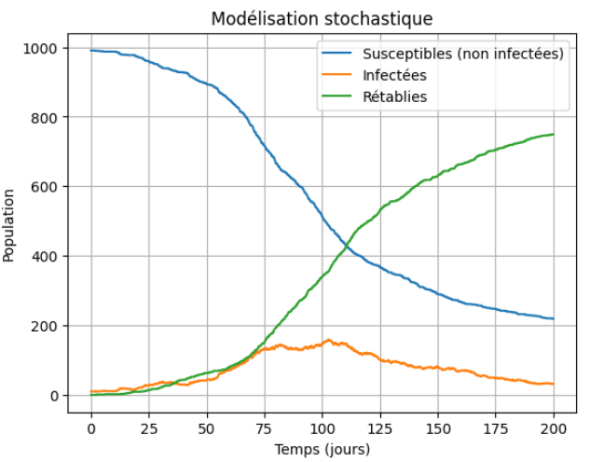
\includegraphics[width=0.45\linewidth, height=0.45\textheight, valign=c]{sir_stochastique}
		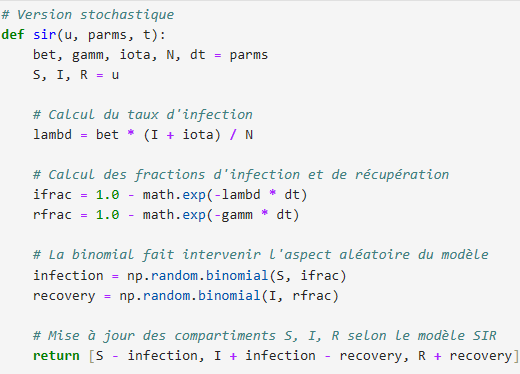
\includegraphics[width=0.5\linewidth, height=0.5\textheight, valign=c]{sir_stochastique_python_1}

        \begin{multicols}{2}
            \begin{itemize}
                    \item $\gamma = 0.05$
                    \item $\beta = 0.1$
                    \item $N = 1000$
                    \item $I_0 = 10$
            \end{itemize}
        \end{multicols}

\end{frame}



